\documentclass[UTF8]{ctexart}
\CTEXsetup[format={\Large\bfseries}]{section}
\usepackage[dvipsnames]{xcolor}
\usepackage{geometry}
\usepackage{listings}
\usepackage{graphicx}

\title{体系结构 Lab4}
\author{PB19000015 贾欣宇}
\date{\today}
\geometry{a4paper,scale=0.75}
\lstset{
    basicstyle          =   \sffamily,          % 基本代码风格
    keywordstyle        =   \bfseries,          % 关键字风格
    commentstyle        =   \rmfamily\itshape,  % 注释的风格,斜体
    stringstyle         =   \ttfamily,  % 字符串风格
    flexiblecolumns,                % 别问为什么,加上这个
    numbers             =   left,   % 行号的位置在左边
    showspaces          =   false,  % 是否显示空格,显示了有点乱,所以不现实了
    numberstyle         =   \zihao{-5}\ttfamily,    % 行号的样式,小五号,tt等宽字体
    showstringspaces    =   false,
    captionpos          =   b,      % 这段代码的名字所呈现的位置,t指的是top上面
    frame               =   lrtb,   % 显示边框
}
\lstdefinestyle{verilog}{
    language        =   verilog, % 语言选Python
    basicstyle      =   \zihao{-5}\ttfamily,
    numberstyle     =   \zihao{-5}\ttfamily,
    keywordstyle    =   \color{blue},
    keywordstyle    =   [2] \color{teal},
    stringstyle     =   \color{magenta},
    commentstyle    =   \color{red}\ttfamily,
    breaklines      =   true,   % 自动换行,建议不要写太长的行
    columns         =   fixed,  % 如果不加这一句,字间距就不固定,很丑,必须加
    basewidth       =   0.5em,
}

\begin{document}
\maketitle
\tableofcontents

\section{实验目的}

\begin{itemize} 
    \item 实现 BTB(Branch Target Buffer)和 BHT(Branch History Table)两种动态分支预测器;
    \item 体会动态分支预测对流水线性能的影响.
\end{itemize}

\section{实验内容}

\subsection{分支预测实现}

根据分支预测方式的选择,分支预测信号 pr 更新如下:

\begin{lstlisting}[style=verilog,caption={更新分支预测信号 pr}]
if(Predict_en == `BTB)
    pr = pr_en & pr_btb;
else if(Predict_en == `BHT)
    pr = pr_en & pr_bht;
else
    pr = 0;  
\end{lstlisting}

其中 pr\_en 为 BTB 命中信号,pr\_btb 为 BTB 预测结果,pr\_bht 为 BHT 预测结果. 当使用 BHT 进行分支预测时,BTB 的预测结果将不被采纳.

分支预测信号 pr 在生成 NPC 和处理 Hazard 中的作用如下:

\begin{lstlisting}[style=verilog,caption={生成 NPC}]
if (br && ~prE) NPC = br_target;
else if (~br && prE) NPC = PCE_4;
else if (jalr) NPC = {jalr_target[31:1], 1'b0};
else if (jal) NPC = jal_target;
else if (prF) NPC = pr_target;
else NPC = PC;
\end{lstlisting}

\begin{lstlisting}[style=verilog,caption={处理 Hazard}]
if ((br && ~prE) || (~br && prE) || jalr)
begin
    bubbleF = 0; flushF = 0;
    bubbleD = 0; flushD = 1;
    bubbleE = 0; flushE = 1;
    bubbleW = 0; flushW = 0;
end
\end{lstlisting}

分支预测的具体实现如下.

\subsubsection{BTB}

\begin{itemize} 
    \item BTB 是一个 1 bit 预测器,如果上次这条分支指令跳转,那么这次它也跳转;如果上次不跳,那么这次也不跳;
    \item BTB 保存当前地址、目标地址、有效位和跳转状态,类似于直接映射的 Cache;
    \item BTB 内容读取在 IF 阶段进行,根据 BTB 是否命中及 BTB 跳转状态信息决定下一条指令的地址;
    \item BTB 根据实际是否跳转和 IF 阶段是否命中的信息,在 EX 阶段修改保存的数据.
\end{itemize}

\begin{lstlisting}[style=verilog,caption={生成 BTB 预测结果}]
pr_target = 0;
pr_en = 0;
pr_btb = 0;
for(integer i = 0; i < 64; i++) begin
    if(PC_IF == prTag[i] && prValid[i]) begin
        pr_target = prTarget[i];
        pr_en = 1;
        pr_btb = prBtb[i];
        break;
    end
end
\end{lstlisting}

以上是 BTB 预测结果的生成,该过程在 IF 阶段一周期内完成.

\begin{lstlisting}[style=verilog,caption={更新 BTB 保存数据}]
if(opE == `B_TYPE) begin
    integer i;
    for(i = 0; i < 64; i++) begin
        if(PC_EX == prTag[i]) begin
            prBtb[i] <= br;
            break;
        end
    end
    if(i == 64 && br) begin
        prTag[pointer] <= PC_EX;
        prTarget[pointer] <= br_target;
        prValid[pointer] <= 1;
        prBtb[pointer] <= 1;
        pointer <= pointer + 1;
    end
end
\end{lstlisting}

以上是 BTB 保存数据的更新,该过程在 EX 阶段一周期内完成. 由于 BTB 存储空间有限,
仅在未记录的跳转指令发生跳转时在 BTB 中加入该指令的记录,如此并不会影响分支预测的结果.

\subsubsection{BHT}

\begin{itemize} 
    \item BHT 存储 2 bit 预测数据,在 IF 阶段进行读取;
    \item BHT 实现一个状态机,在 EX 阶段根据状态机更新预测数据;
    \item BHT 每项存储的数据量很小,因此其存储项目数可以远大于 BTB.
\end{itemize}

\begin{lstlisting}[style=verilog,caption={生成 BHT 预测结果}]
assign pr_bht = prBht[tagIF][1];
\end{lstlisting}

BHT 使用指令 [9:2] 位对应存储地址的预测数据的高位作为分支预测结果.

\begin{lstlisting}[style=verilog,caption={更新 BHT 保存数据}]
if(opE == `B_TYPE) begin
    if(br) begin
        prBht[tagEX] <= (prBht[tagEX] == 2'b11) ? 2'b11 : prBht[tagEX] + 2'b01;
    end
    else begin
        prBht[tagEX] <= (prBht[tagEX] == 2'b00) ? 2'b00 : prBht[tagEX] - 2'b01;
    end
end
\end{lstlisting}

BHT 实现了如图 \ref{bht} 的状态机来更新预测数据(自 01 状态即 weakly not taken 状态启动).

\begin{figure}[htbp]
\centering
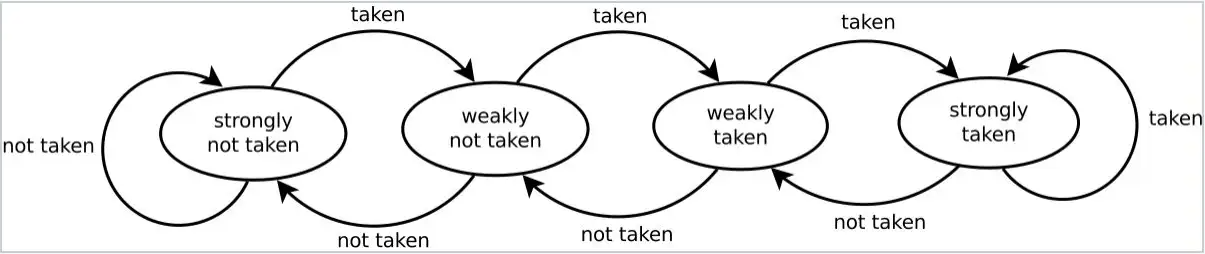
\includegraphics[width = .85\textwidth]{1.png}
\caption{BHT 状态机}
\label{bht}
\end{figure}

\subsection{实验分析}

分别对四组样例(BTB、BHT、快速排序、矩阵乘法)使用 BTB 和 BHT 分支预测方案进行测试,并测试一组无预测情况作为对比,结果如表 \ref{fx}.

\begin{table}[htbp]
\centering
\begin{tabular}{l|r r r r}
 \hline
样例 & BTB & BHT & 快速排序 & 矩阵乘法 \\
 \hline
分支收益(周期) & 2 & 2 & 2 & 2 \\
分支代价(周期) & 2 & 2 & 2 & 2 \\
总周期数(无预测) & 511 & 537 & 35,616 & 71,504 \\
总周期数(BTB) & 315 & 383 & 36,116 & 63,900 \\
总周期数(BHT) & 315 & 365 & 34,586 & 63,360 \\
周期数差值(BTB) & 196 & 154 & -500 & 7,604 \\
周期数差值(BHT) & 196 & 172 & 1,030 & 8,144 \\
分支指令数 & 101 & 110 & 6,633 & 4,624 \\
分支指令执行数 & 100 & 99 & 1,698 & 4,350 \\
预测正确数(BTB) & 99 & 88 & 4,685 & 4,076 \\
预测正确数(BHT) & 99 & 97 & 5,450 & 4,346 \\
预测错误数(BTB) & 2 & 22 & 1,948 & 548 \\
预测错误数(BHT) & 2 & 13 & 1,183 & 278 \\
 \hline
\end{tabular}
\caption{实验结果统计}
\label{fx}
\end{table}

由于测试次数很多,选取 BTB 样例的无预测测试和矩阵乘法样例的 BHT 测试结果如图 \ref{t2}、图 \ref{t3} 所示. 由测试结果可知:

\begin{itemize} 
    \item 分支收益和分支代价与具体样例无关,只与 CPU 设计有关;
    \item 若预测错误次数过多,使用分支预测时的性能可能反而劣于未使用分支预测时;
    \item 对每种分支预测方案,$\mbox{周期数差值}=(\mbox{分支指令执行数}-\mbox{预测错误数})*\mbox{分支代价}$;
    \item 对 BTB 方案,$\mbox{预测错误数}=\mbox{循环个数}*2$,对 BHT 方案,$\mbox{预测错误数}=\mbox{循环个数}+\mbox{循环种数}$;
    \item BHT 方案预测错误数较少、运行总周期数较少、性能较优.
\end{itemize}

\begin{figure}[htbp]
\centering
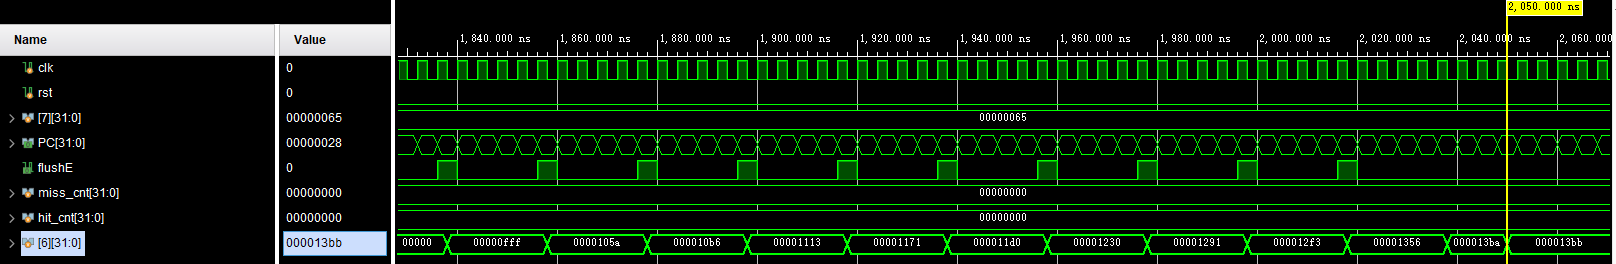
\includegraphics[width = .85\textwidth]{2.png}
\caption{BHT 状态机}
\label{t2}
\end{figure}

\begin{figure}[htbp]
\centering
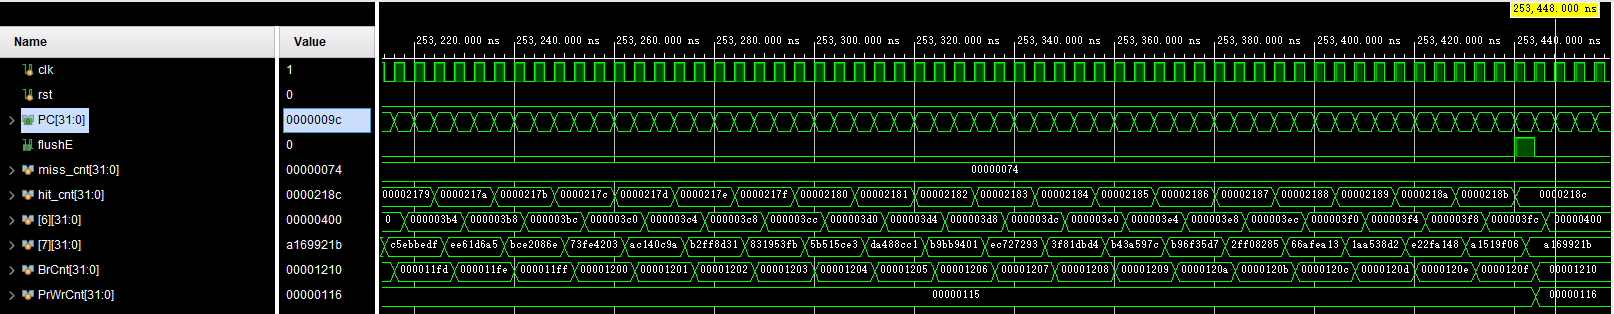
\includegraphics[width = .85\textwidth]{3.png}
\caption{BHT 状态机}
\label{t3}
\end{figure}

\section{实验总结}

本次实验中完成了 BTB 和 BHT 分支预测器的设计,并通过测试体会了二者对流水线性能的影响,加深了对分支预测的理解.

\end{document}
